This chapter describes the in the experiments used hardware and software.  
\section{Hardware} \label{sec:Hardware}
\subsection{High-speed Cameras}

\todo{cams - their specs (lenses as well) - color vs. speed, speed vs. quality/ memory}
high-speed vs. normal cams --> auf versuch verweisen

the recorded data uses a lot of memory!!!

\subsection{External Trigger}\label{ssec:ExTrigger}
\todo{write stuff - find documentation, whats its name?}\\

\begin{figure}[htbp]
		\centering
		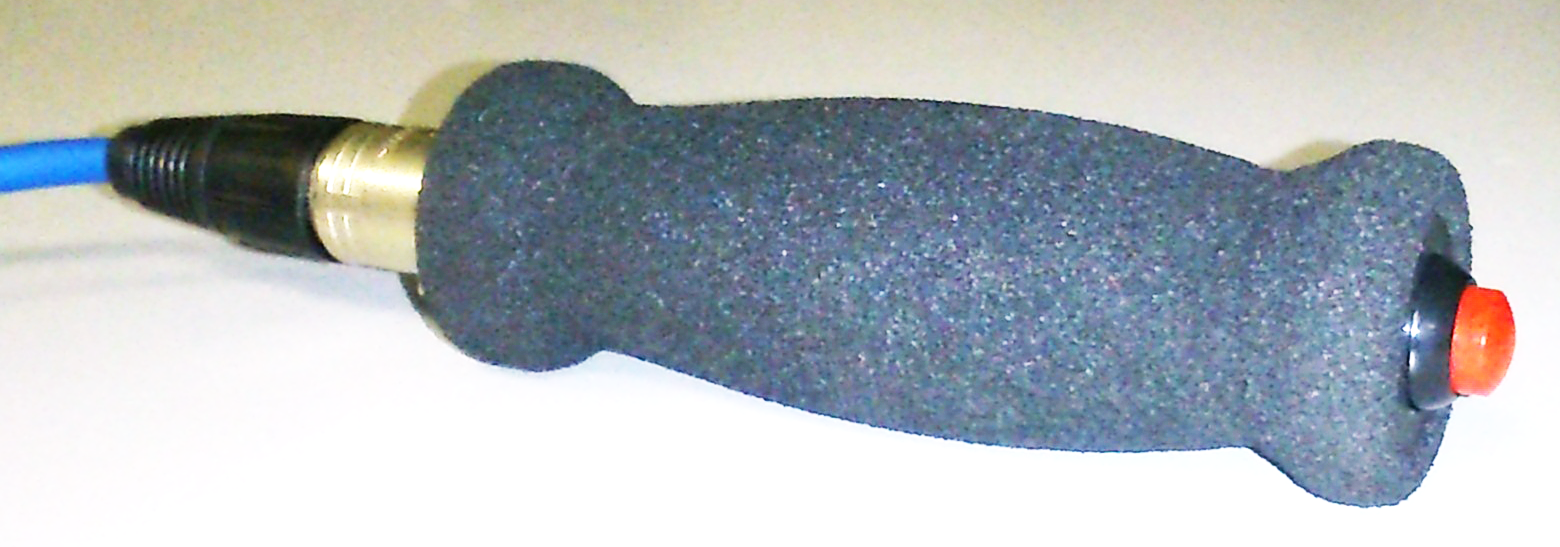
\includegraphics[width=1.0\textwidth]{figures/Trigger}
		\caption[External trigger]{The external trigger.}
		\label{fig:ExTrigger}
\end{figure}

\subsection{Lighting}

\subsection{Calibration Pattern}
calibration pattern: checkerboard
first big one (durchmesser): appendix or: \url{http://www.vision.caltech.edu/bouguetj/calib_doc/htmls/pattern.pdf}
then smaller, finer one (durchmesser)


\section{Software} \label{sec:Software}
This thesis was written in \LaTeX . Other software used is explained in the following sections.

\subsection{Timebench} \label{ssec:Timebench}
The software \textit{TimeBench}\footnote{More information about TimeBench can be found on the official website at \url{http://www.optronis.com/en/products/high-speed-cameras/software.html}.} was developed by \textit{Optronis} and is included in the delivery of their high-speed camera series. It lets the user record high-speed image sequences and comes with several tools to adjust, analyze and export these sequences (\cite{Optronis.2016}). 

The software was chosen because of its close connection to the used high-speed cameras.

TimeBench should be only started after the two high-speed cameras have been already installed, otherwise the cameras may not be recognized by the software. The two cameras need to be dragged into a \textit{synchronization group} 

\begin{figure}[htbp]
		\centering
		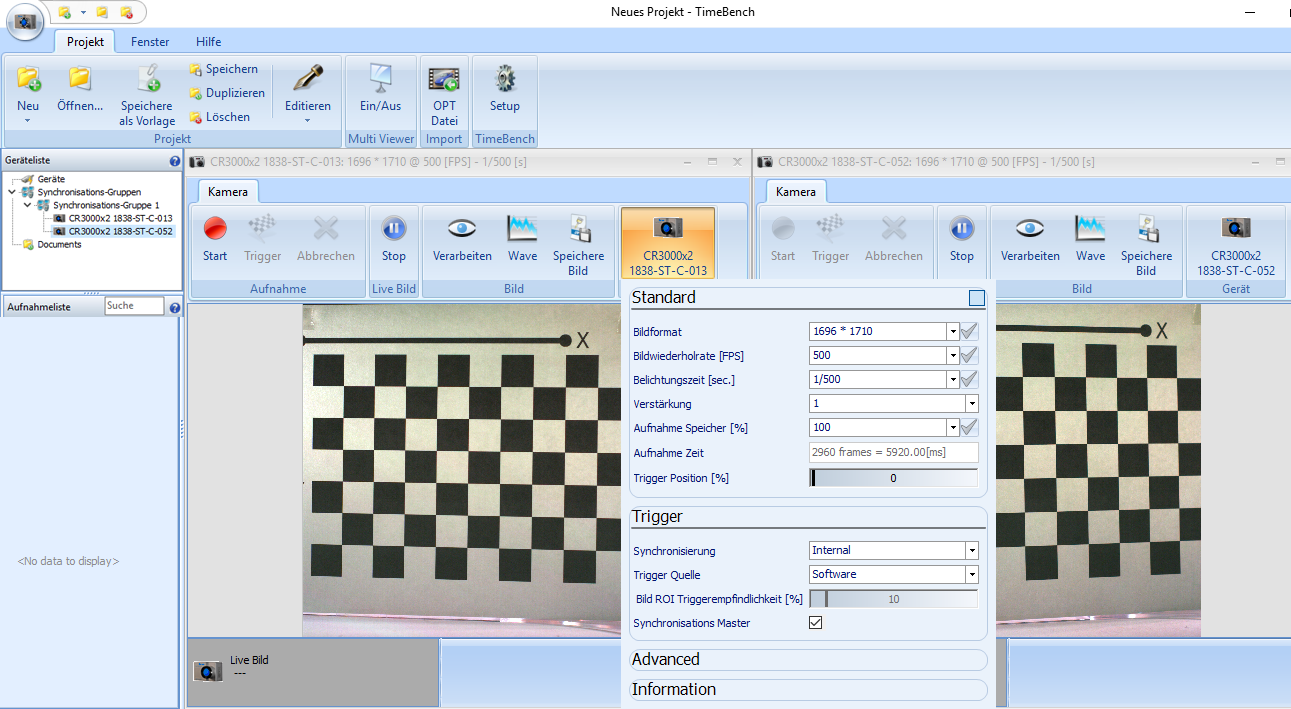
\includegraphics[width=1.0\textwidth]{figures/timebenchRecord}
		\caption[The views of two synchronized cameras and their recording options in TimeBench]{The views of two synchronized cameras and their recording options in TimeBench (\textit{source: software TimeBench owned by} \cite{Optronis.2016}).}
		\label{fig:timebanchRecord}
\end{figure}

The software was first used to create image pair sequences of the calibration patter in several positions and angles for the camera calibration process (see \autoref{ssec:calibration}). And then it was used for recording a high-speed image sequence of moving objects to later reconstruct them in MATLAB (see \autoref{ssec:reconstruction}). 
\todo{reference to experiment cam calibration and reconstructing of objects}\\

Either scan anleitung or find it online and include it on cd!

\subsection{MATLAB} \label{ssec:Matlab}
For the camera calibration as well as for the 3-D reconstruction, the commercial platform \textit{MATLAB}\index{MATLAB} by \textit{MathWorks} was used. MATLAB is a software that is specialized in solving mathematical problems (especially matrix operations) and visualizing data. The MATLAB programming language is matrix-based and implements object-oriented concepts like classes and inheritance. The program comes with a large library of built-in toolboxes, which can be used to address many different engineering and scientific problems. Another of MATLAB's strengths lies with its active community, which provides costum scripts and discusses recent developments in the scientific field (\cite{MathWorks.2016}).

A large portion of the MATLAB community is involved in researching the algorithms that drive the field of multiple view geometry in computer vision (see \autoref{c:relatedWorks} for examples). MathWorks also implements new content on this topic regularly. 

The reasons stated above led to the usage of MATLAB as the development environment of choice in this thesis. Initially MATLAB R2015b was used, but due to newly added functions for data refinement (see \autoref{sec:refinement}) the software needed to be updated to MATLAB R2016a.
   
The 3-D reconstruction was programmed and organized in one MATLAB script file. To get the needed stereo parameters an built-in toolbox was used, which will be discussed in the following sections. Documentation for all functions used and a step-by-step-guide can be found in \autoref{c:Implementation}.

One of the biggest problems with MATLAB is its documentation. Although it often provides good examples and a lot of details, it is not explicit enough in other important areas. Certain algorithms used in the built-in functions are often times not explained, making it difficult to find mistakes when the data output is unexpected\footnote{This \enquote{blackbox} problem with which you can not see how the output is created may be owed to the fact that MATLAB is (and is used as) a commercial software.}. The toolboxes often lack information as well, for example an explanation of how the pipelines work, which coordinate system is used, etc. These problems restrict the programmer quite a bit and force one to either find a work around or use third party programs. More details on the encountered problems can be found in the following chapters (especially \autoref{sec:Calibration} and \todo{add all chapters with big probs here}).

\subsubsection{Camera Vision Toolbox}
its coordinate systems: \url{http://www.mathworks.com/help/vision/gs/coordinate-systems.html}
\subsubsection{Camera Calibration Toolbox for MATLAB}
good for double checks, may also be used as a tutorial on camera calibration since it includes general information about calibration, references and related links

release: \url{http://www.vision.caltech.edu/bouguetj/calib_doc/}
example: \url{http://www.vision.caltech.edu/bouguetj/calib_doc/htmls/example.html}

\subsubsection{Stereo calbr. toolbox for matlab}
stereoParameters classs
intrinsics
extrisics


\section{Experiment architecture} \label{sec:architecture}
endgültiger versuchsaufbau, many different before, which will be mentioned in the experimental phase --> visualize pipeline (?) + tatsächliche architecture

\note{Aufbau cameras, konvergierend etc.. siehe hinweis Luhman p.194 and 295}